\documentclass[a4paper,11pt, twoside]{article}
\newcommand{\n}[1]{\textbf{#1}}
\usepackage{graphicx}
\usepackage{amsfonts}
\usepackage{amsmath}
\usepackage[brazilian]{babel}
\usepackage[utf8]{inputenc}
\usepackage[T1]{fontenc}
\usepackage {multirow}
\usepackage {booktabs}
\usepackage {fancyhdr}
\usepackage {graphicx}
\usepackage{xcolor}
\linespread {1.5}
\date{\today}
\author{Caio Vinícius Dadauto - 7994808}
\title{Exercicío de Programa 1}
\usepackage{listings}
\lstset{numbers=left,
stepnumber=1,
firstnumber=1,
numberstyle=\tiny,
extendedchars=false,
breaklines=flase,
tabsize=2,
showtabs=true,
tab=\textcolor{gray}{$\cdots$},
frame=tb,
basicstyle=\footnotesize,
stringstyle=\ttfamily,
showstringspaces=false}
\renewcommand{\lstlistingname}{Programa}
\renewcommand{\lstlistlistingname}{Lista de Listagens}
\begin{document}
    \pagestyle{fancy}
    \fancyhf{}
    \renewcommand{\footrulewidth}{0.1pt}
    \renewcommand{\headrulewidth}{0.0pt}
    \fancyfoot[LE, RO]{\bfseries \thepage}

    \begin{center}
        \begin{tabular}{c}
            {\huge Exercício de Programa 2}\\[-0.5cm]
            \rule{0.6\textwidth}{0.1mm}\\
            Caio Vnícius Dadauto$\quad$7994808\\
            {\small 23 de abril de 2013}
        \end{tabular}
    \end{center}
    \vspace{2cm}

    \section*{Item A}
    \begin{figure}[!ht]
        \begin{center}
            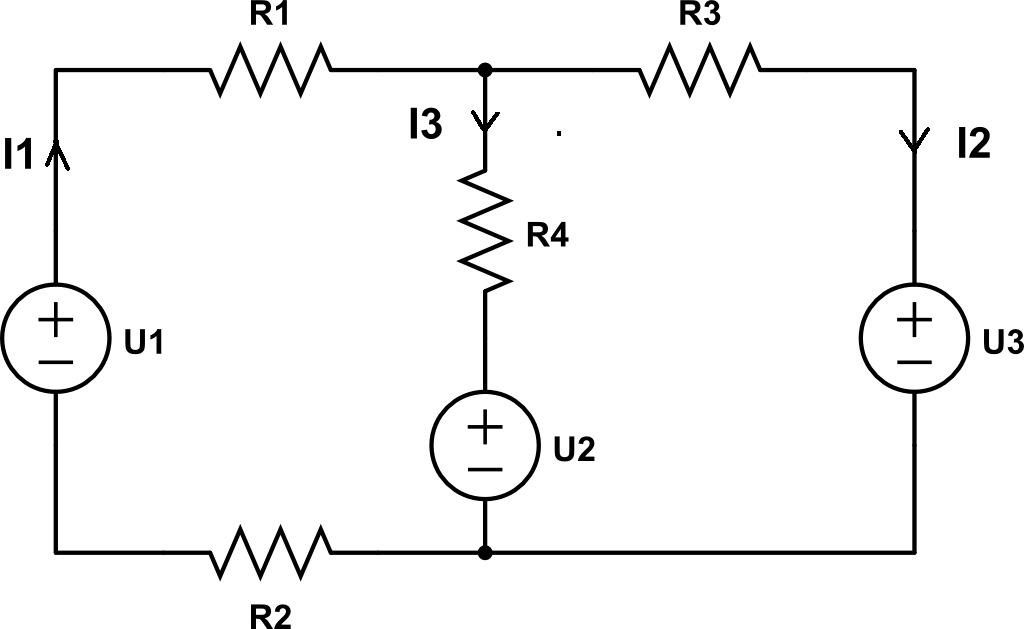
\includegraphics[scale=0.25]{circ.jpg}
        \end{center}
        \caption{Circuito A.\label{A}}
    \end{figure}

    Aplicando Kirchhoff ao circuito A se obtem as seguintes relações.
    \begin{eqnarray}
        U_1 - I_1R_1 - I_3R_4 - U_2 - I_1R_2 & = & 0\\
        U_3 + I_2R_3 - I_3R_4 - U_4 & = & 0\\
        I_1 - I_2 - I_3 & = & 0
    \end{eqnarray}
    Onde $R_1 = 5\Omega$, $R_2 = 7\Omega$, $R_3 = 5\Omega$, $R_4 = 2\Omega$,
    $U_1 = 24V$, $U_2 = 24V$ e $U_3 = 24V$.

    A partir das relações apresentadas acima, tem-se o seguinte sistema:
    \begin{equation}\label{sist}
        \left \{ \begin{array}{c c c}
                12I_1 - 2I_3 & = & 15\\
                5I_2 - 2I_3 & = & 3\\
                I_1 - I_2 - I_3 & = & 0
                \end{array} \right .
    \end{equation}
    que na forma matricial é dado por:
    \begin{displaymath}
        \left [\begin{array}{c c c}
                    12 & 0 & 2\\
                    0 & 5 & 2\\
                    1 & -1 & -1
                \end{array} \right ]
        \left [\begin{array}{c}
                    I_1\\
                    I_2\\
                    I_3
                 \end{array} \right ]
        =
        \left [\begin{array}{c}
                    15\\
                    3\\
                    0
                \end{array} \right ]
    \end{displaymath}
    
    \subsection*{Item B}
    Tendo em vista a solução do sistema apresentado no item A e, ainda, a solução de qualquer sistema
    de n equações e n variaveis, é possível implementar um programa para determinar tal solução.
    Programa que utiliza do método de eliminação de Gauss com pivotação parcial.
    O programa trabalha com $n < 100$ e matrizes que nao possuem fileiras nulas (colunas ou linhas).
    
    {\linespread{1.15}
    \lstinputlisting[language=C, label=sqlselect, caption={Implementação para solução 
    de sistemas pelo método de Gauss.}]{eli_gauss.c}}
    
    Inserindo como entrada do programa acima a matriz expandida do sistema \eqref{sist}, obtem-se o
    seguinte conjunto de matrizes para cada etapa de eleminação;
    
    Etapa 1:
    \[
        \left [\begin{array}{c c c c}
                    12.00000    &   0.00000 &   2.00000 &   15.00000\\
                    0.00000 &   5.00000 &   -2.00000    &   3.00000\\
                    1.00000 &   -1.00000    &   -1.00000    &   0.00000\\
                \end{array} \right ]
    \]
    
    Etapa 2:
    \[
        \left [\begin{array}{c c c c}
                    12.00000    &   0.00000 &   2.00000 &   15.00000\\
                    0.00000 &   5.00000 &   -2.00000    &   3.00000\\
                    0.00000 &   -1.00000    &   -1.16667    &   -1.25000\\
                \end{array} \right ]
    \]
    
    Etapa 3:
        \[
        \left [\begin{array}{c c c c}
                    12.00000    &   0.00000 &   2.00000 &   15.00000\\
                    0.00000 &   5.00000 &   -2.00000    &   3.00000\\
                    0.00000 &   0.00000 &   -1.56667    &   -0.65000\\
                \end{array} \right ]
    \]
    
    obtendo como solução:
    \[
     I_1 =  1.18085A\quad I_2 = 0.76596A\quad I_3 = 0.41489A
    \]
    
    \subsection*{Item C}
    Tendo em vista solucionar o mesmo sistema do item A, porém agora utilizando do
    método de Jacobi, é necessário que a matriz dos coeficientes do sistema \eqref{sist}
    satisfaça o critério das linhas, dado por:
    \begin{equation}
        \sum^n_{j = 1} \frac{|a_{kj}|}{|a_{kk}|} < 1,\quad\mathrm{j \ne k}
    \end{equation}
    onde $a$ é o elemento de linha $k$ e coluna $j$ da matriiz dos coeficientes.
    Para isso as duas primeiras linhas do sistema \eqref{sist} precisam ser trocadas,
    antes de ser aplicado o método de Jacobi. Obtendo a seguinte matriz expandida:
    \begin{equation}\label{mat}
        \left [\begin{array}{c c c c}
                    12.000  &   0.000   &   2.000   &   15.000\\
                    0.000   &   5.000   &   -2.000  &   3.000\\
                    1.000   &   -1.000  &   -1.000  &   0.000
                \end{array} \right ]
    \end{equation}
    
    Segue abaixo o programa que implementa o método de Jacobi.
    
    {\linespread{1.15}
    \lstinputlisting[language=C, label=sqlselect, caption={Implementação para o método de Jacobi.}]{jacobi.c}}
    
    É apresentado na tabela \ref{tab} os valores das soluções aproximadas geradas a cada interação pelo programa 2 para a matriz \eqref{mat}.
    
    {\linespread{1}
    \begin{table}[!th]
        \begin{center}
            \begin{tabular}{ c c c c c c c }
                \toprule[0.11em]
                \n{Interação (k)} & \n{$I_1^{(k)}$} & \n{$I_2^{(k)}$} & \n{$I_3^{(k)}$} & \n{$erro_1^{(k)}$} & \n{$erro_2^{(k)}$} & \n{$erro_3^{(k)}$}\\
                \toprule[0.11em]
                0 & 1.00000 & 1.00000 & 1.00000 & $\cdots$  &  $\cdots$  &  $\cdots$ \\
                \midrule
                1 & 1.08333 & 1.00000 & 0.00000 & 0.08333  & 0.00000  & 1.00000 \\
                \midrule
                2 & 1.25000 & 0.60000 & 0.08333 & 0.16667  & 0.40000  & 0.08333 \\
                \midrule
                3 & 1.23611 & 0.63333 & 0.65000 & 0.01389  & 0.03333  & 0.56667 \\
                \midrule
                4 & 1.14167 & 0.86000 & 0.60278 & 0.09444  & 0.22667  & 0.04722 \\
                \midrule
                5 & 1.14954 & 0.84111 & 0.28167 & 0.00787  & 0.01889  & 0.32111 \\
                \midrule
                6 & 1.20306 & 0.71267 & 0.30843 & 0.05352  & 0.12844  & 0.02676 \\
                \midrule
                7 & 1.19860 & 0.72337 & 0.49039 & 0.00446  & 0.01070  & 0.18196 \\
                \midrule
                8 & 1.16827 & 0.79616 & 0.47523 & 0.03033  & 0.07279  & 0.01516 \\
                \midrule
                9 & 1.17080 & 0.79009 & 0.37211 & 0.00253  & 0.00607  & 0.10311 \\
                \midrule
                10 & 1.18798 & 0.74885 & 0.38071 & 0.01719  & 0.04124  & 0.00859 \\
                \midrule
                11 & 1.18655 & 0.75228 & 0.43914 & 0.00143  & 0.00344  & 0.05843 \\
                \midrule
                12 & 1.17681 & 0.77565 & 0.43427 & 0.00974  & 0.02337  & 0.00487 \\
                \midrule
                13 & 1.17762 & 0.77371 & 0.40116 & 0.00081  & 0.00195  & 0.03311 \\
                \midrule
                14 & 1.18314 & 0.76046 & 0.40392 & 0.00552  & 0.01324  & 0.00276 \\
                \midrule
                15 & 1.18268 & 0.76157 & 0.42268 & 0.00046  & 0.00110  & 0.01876 \\
                \midrule
                16 & 1.17955 & 0.76907 & 0.42111 & 0.00313  & 0.00751  & 0.00156 \\
                \midrule
                17 & 1.17981 & 0.76845 & 0.41048 & 0.00026  & 0.00063  & 0.01063 \\
                \midrule
                18 & 1.18159 & 0.76419 & 0.41137 & 0.00177  & 0.00425  & 0.00089 \\
                \midrule
                19 & 1.18144 & 0.76455 & 0.41739 & 0.00015  & 0.00035  & 0.00602 \\
                \midrule
                20 & 1.18043 & 0.76696 & 0.41689 & 0.00100  & 0.00241  & 0.00050 \\
                \midrule
                21 & 1.18052 & 0.76676 & 0.41348 & 0.00008  & 0.00020  & 0.00341 \\
                \midrule
                \multicolumn{7}{r}{{\small Continuação na proxima página.}}\\
                \midrule
            \end{tabular}
        \end{center}
    \end{table}}
    
    {\linespread{1}
    \begin{table}[!th]
        \begin{center}
            \begin{tabular}{ c c c c c c c }
                \midrule
                \multicolumn{7}{l}{{\small Continuação da página anterior.}}\\
                \midrule
                22 & 1.18109 & 0.76539 & 0.41376 & 0.00057  & 0.00137  & 0.00028 \\
                \midrule
                23 & 1.18104 & 0.76550 & 0.41570 & 0.00005  & 0.00011  & 0.00193 \\
                \midrule
                24 & 1.18072 & 0.76628 & 0.41554 & 0.00032  & 0.00077  & 0.00016 \\
                \midrule
                25 & 1.18074 & 0.76621 & 0.41444 & 0.00003  & 0.00006  & 0.00110 \\
                \midrule
                26 & 1.18093 & 0.76578 & 0.41453 & 0.00018  & 0.00044  & 0.00009 \\
                \midrule
                27 & 1.18091 & 0.76581 & 0.41515 & 0.00002  & 0.00004  & 0.00062 \\
                \midrule
                28 & 1.18081 & 0.76606 & 0.41510 & 0.00010  & 0.00025  & 0.00005 \\
                \midrule
                29 & 1.18082 & 0.76604 & 0.41475 & 0.00001  & 0.00002  & 0.00035 \\
                \midrule
                30 & 1.18088 & 0.76590 & 0.41478 & 0.00006  & 0.00014  & 0.00003 \\
                \midrule
                31 & 1.18087 & 0.76591 & 0.41498 & 0.00000  & 0.00001  & 0.00020 \\
                \midrule
                32 & 1.18084 & 0.76599 & 0.41496 & 0.00003  & 0.00008  & 0.00002 \\
                \toprule[0.11em]
                \multicolumn{7}{c}{\n{Solução aproximada}}\\
                \toprule[0.11em]
                \multicolumn{7}{c}{$I_1 = 1.18084A\quad I_2 = 0.76599A\quad I_3 = 0.41496A$}\\
                \midrule
            \end{tabular}
        \end{center}
        \caption{Resultados obtidos pelo método de Jacobi.}\label{tab}
    \end{table}}
    
    \subsection*{Item C}
    Partindo do mesmo sistema \eqref{sist}, mas agoro utilizando o método de Gauss-Seidel
    para a solução do mesmo, há a necessidade de satisfazer o critério de Sassenfeld que é
    dado por:
    \begin{equation}
        \beta = \mathrm{max}_{1 \le i \le n} \;\{\beta_i\} < 1
    \end{equation}
    onde,
    \[
        \beta_i = \frac{\sum^{i - 1}_{j = 1}\beta_j|a_{ij}| + \sum^n_{j = i + 1}|a_{ij}|}{|a_{ii}|}
    \]
    sendo que a matriz expandiada \eqref{mat} satisfaz tal critério.
    
    Segue o código para solucionar a matriz \eqref{mat} pelo métodode Gauss-Seidel.
    
    {\linespread{1.15}
    \lstinputlisting[language=C, label=sqlselect, caption={Implementação para o método de Jacobi.}]{seidel.c}}
    \newpage
    É apresentado na tabela \ref{tab1} os valores das soluções aproximadas geradas a cada interação pelo programa 3 para a matriz \eqref{mat}.

    {\linespread{1}
    \begin{table}[!th]
        \begin{center}
            \begin{tabular}{ c c c c c c c }
                \toprule[0.11em]
                \n{Interação (k)} & \n{$I_1^{(k)}$} & \n{$I_2^{(k)}$} & \n{$I_3^{(k)}$} & \n{$erro_1^{(k)}$} & \n{$erro_2^{(k)}$} & \n{$erro_3^{(k)}$}\\
                \toprule[0.11em]
                0 & 1.00000 & 1.00000 & 1.00000 & $\cdots$  & $\cdots$  & $\cdots$ \\
                \midrule
                1 & 1.08333 & 1.00000 & 0.08333 & 0.08333  & 0.00000  & 0.91667 \\
                \midrule
                2 & 1.23611 & 0.63333 & 0.60278 & 0.15278  & 0.36667  & 0.51944 \\
                \midrule
                3 & 1.14954 & 0.84111 & 0.30843 & 0.08657  & 0.20778  & 0.29435 \\
                \midrule
                4 & 1.19860 & 0.72337 & 0.47523 & 0.04906  & 0.11774  & 0.16680 \\
                \midrule
                5 & 1.17080 & 0.79009 & 0.38071 & 0.02780  & 0.06672  & 0.09452 \\
                \midrule
                6 & 1.18655 & 0.75228 & 0.43427 & 0.01575  & 0.03781  & 0.05356 \\
                \midrule
                7 & 1.17762 & 0.77371 & 0.40392 & 0.00893  & 0.02142  & 0.03035 \\
                \midrule
                8 & 1.18268 & 0.76157 & 0.42111 & 0.00506  & 0.01214  & 0.01720 \\
                \midrule
                9 & 1.17981 & 0.76845 & 0.41137 & 0.00287  & 0.00688  & 0.00975 \\
                \midrule
                10 & 1.18144 & 0.76455 & 0.41689 & 0.00162  & 0.00390  & 0.00552 \\
                \midrule
                11 & 1.18052 & 0.76676 & 0.41376 & 0.00092  & 0.00221  & 0.00313 \\
                \midrule
                12 & 1.18104 & 0.76550 & 0.41554 & 0.00052  & 0.00125  & 0.00177 \\
                \midrule
                13 & 1.18074 & 0.76621 & 0.41453 & 0.00030  & 0.00071  & 0.00100 \\
                \midrule
                14 & 1.18091 & 0.76581 & 0.41510 & 0.00017  & 0.00040  & 0.00057 \\
                \midrule
                15 & 1.18082 & 0.76604 & 0.41478 & 0.00009  & 0.00023  & 0.00032 \\
                \midrule
                16 & 1.18087 & 0.76591 & 0.41496 & 0.00005  & 0.00013  & 0.00018 \\
                \midrule
                17 & 1.18084 & 0.76598 & 0.41486 & 0.00003  & 0.00007  & 0.00010 \\
                \midrule
                18 & 1.18086 & 0.76594 & 0.41491 & 0.00002  & 0.00004  & 0.00006 \\
                \toprule[0.11em]
                \multicolumn{7}{c}{\n{Solução aproximada}}\\
                \toprule[0.11em]
                \multicolumn{7}{c}{$I_1 = 1.18086A\quad I_2 = 0.76594A\quad I_3 = 0.41491A$}\\
                \midrule
            \end{tabular}
        \end{center}
        \caption{Resultados obtidos pelo método de Gauss-Seidel.}\label{tab1}
    \end{table}}
    
\end{document}